% !TEX root = saveliev_physics_general_course_2.tex
%!TEX TS-program = pdflatex
%!TEX encoding = UTF-8 Unicode


\chapter[CHUYỂN ĐỘNG CỦA ĐIỆN TÍCH TRONG ĐIỆN TRƯỜNG\\
VÀ TỪ TRƯỜNG]{CHUYỂN ĐỘNG ỦA ĐIỆN TÍCH \\TRONG ĐIỆN TRƯỜNG\\ VÀ TỪ TRƯỜNG}\label{chap:10}
\chaptermark{MOTION OF CHARGED PARTICLES}

\section{Chuyển động của điện tích trong từ trường}\label{sec:10_1}

Xét một hạt điện tích $e'$ chuyển động trong từ trường đều với vận tốc $\vec{v}$ vuông góc với $\vec{B}$.
Lực từ tác dụng tác dụng lên điện tích một gia tốc vuông góc với vận tốc
\begin{equation}\label{eq:10_1}
    \ab{a}{n} = \frac{F}{m} = \frac{e'}{m} vB
\end{equation}

\noindent
[xem \eqn{6_33}; $\vec{v}$ và $\vec{B}$ vuông góc với nhau].
Gia tốc này chỉ thay đổi hướng của vận tốc và giữ nguyên độ lớn.
Do đó, gia tốc đưa ra bởi \eqn{10_1} sẽ giữ nguyên độ lớn.
Trong những điều kiện này, hạt sẽ chuyển động tròn đều với bán kính được xác định bởi công thức $\ab{a}{n}=v^2/R$.
Thế giá trị $\ab{a}{n}$ tại \eqn{10_1} vào phương trình này và giải phương trình theo $R$, ta có
\begin{equation}\label{eq:10_2}
    R = \frac{m}{e'} \frac{v}{B}.
\end{equation}

Do đó, khi một hạt tích điện chuyển động trong một từ trường đều vuông góc với mặt phẳng của chuyển động, quỹ đạo của hạt là một đường tròn.
Bán kính đường trong này phụ thuộc vào vận tốc hạt, cường độ cảm ứng từ và tỉ số của điện tích $e'$ so với khối lượng $m$.
Tỉ số $e'/m$ được gọi là \textbf{điện tích riêng}.

Để tìm chu kỳ $T$ cho chuyển động tròn của hạt điện tích,
ta lấy chu vi đường tròn $2\pi R$ chia cho vận tốc điện tích $v$. Kết quả là
\begin{equation}\label{eq:10_3}
    T = 2\pi \frac{m}{e'} \frac{1}{B}.
\end{equation}

\noindent
Biện luận kết quả \eqn{10_3} cho thấy chu kỳ quay của hạt điện tích không phụ thuộc vào vận tốc. 
Nó chỉ phụ thuộc vào điện tích riêng và cường độ cảm ứng từ.

Xét chuyển động của hạt tích điện khi vận tốc tạo góc $\alpha$ với hướng của từ trường đều, và  $\alpha$ không phải góc vuông.
Ta phân tích $\vec{v}$ thành hai thành phần : $\vec{v}_{\perp}$ vuông góc với $\vec{B}$, và  $\vec{v}_{\parallel}$ song song với to $\vec{B}$ (\fig{10_1}).
Độ lớn của các thành phần này là
\begin{equation*}
    v_{\perp} = v\sin\alpha,\quad v_{\parallel}=v\cos\alpha.
\end{equation*}

Lực từ có độ lớn
\begin{equation*}
    F = e' v B \sin\alpha = e' v_{\perp} B,
\end{equation*}

\noindent
và nằm trong mặt phẳng vuông góc với $\vec{B}$.
Gia tốc gây ra bởi lực này vuông góc với thành phần $\vec{v}_{\perp}$.
Thành phần của lực từ theo hướng của $\vec{B}$ bằng không.
Do đó lực này không thể ảnh hưởng tới độ lớn của $\vec{v}_{\parallel}$.
Do đó chuyển động hạt tích điện khi này có thể xem là chồng chập của hai chuyển động: (1) tịnh tiến dọc theo hướng của $\vec{B}$ với vận tốc không đổi $v_{\parallel}=v\cos\alpha$, và (2) chuyển động tròn đều trong mặt phẳng vuông góc với vector $\vec{B}$

\begin{figure}[t]
	\begin{minipage}[t]{0.48\linewidth}
		\begin{center}
			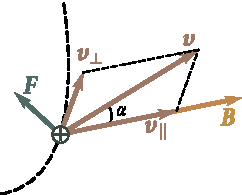
\includegraphics[scale=1]{figures/ch_10/fig_10_1.pdf}
			\caption[]{}
			\label{fig:10_1}
		\end{center}
	\end{minipage}
	\hfill{ }%space{-0.05cm}
	\begin{minipage}[t]{0.48\linewidth}
		\begin{center}
			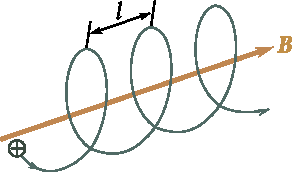
\includegraphics[scale=1]{figures/ch_10/fig_10_2.pdf}
			\caption[]{}
			\label{fig:10_2}
		\end{center}
	\end{minipage}
\vspace{-0.4cm}
\end{figure}

Bán kính đường tròn được xác định bởi \eqn{10_2} với $v_{\perp} = v\sin\alpha$ thay thế cho $v$.
Quỹ đạo chuyển động là một đường xoắn ốc với trục trùng với hướng của $\vec{B}$ (\fig{10_2}).
Bước của đường xoắn ốc này $l$ có thể tìm được bằng cách nhân $v_{\parallel}$ với chuy kỳ quay  $T$ tìm được bởi \eqn{10_3}:
\begin{equation}\label{eq:10_4}
    l = v_{\parallel} T = 2\pi \frac{m}{e'} \frac{1}{B} v \cos\alpha.
\end{equation}
Hướng xoắn của đường xoắn ốc phụ thuộc vào dấu của điện tích.
Nếu là dương, quỹ đạo xoắn ngược chiều kim đồng hồ.
Quỹ đạo của một điện tích âm sẽ xoắn cùng chiều kim đồng hồ (giả thiết rằng ta đang nhìn đường xoắn ốc theo chiều của $\vec{B}$; hạt sẽ chuyển động ra xa ta nếu $\alpha<\pi/2$, và lại gần nếu $\alpha>\pi/2$).

\section{Sự chệch hướng của hạt tích điện 
do điện trường và từ trường}\label{sec:10_2}

Xem xét một chùm tia nhỏ những điện hạt mang điện giống nhau (chẳng hạn như electron) đập vào một màn vuông góc với chùm tại điểm O khi không có xuất hiện các trường (\fig{10_3}).
Hãy xét độ dịch chuyển của vết chùm tia trên màn gây ra bởi một điện trường đều vuông góc (với chùm tia) và tác dụng trên một đoạn đường chiều dài $l_1$.
Đặt vận tốc đầu của hạt là $\vec{v}_0$.
Khi vào vùng có trường, mỗi hạt sẽ chịu một gia tốc đều về cường độ và hướng $a_{\perp}=(e'/m)E$ và vuông góc với $\vec{v}_0$ (tại đây, $e'/m$ là điện tích riêng của hạt).
Chuyển động dưới tác dụng của trường sẽ diễn ra trong thời gian $t = l_1/v_0$.
Trong thời gian này, hạt sẽ bị lệch một đoạn
\begin{equation}\label{eq:10_5}
    y_1 = \frac{1}{2} a_{\perp} t^2 = \frac{1}{2} \frac{e'}{m} E \frac{l_1^2}{v_0^2},
\end{equation}

\noindent
và sẽ có được thành vận tốc $\vec{v}_0$:
\begin{equation*}
    v_{\perp} = a_{\perp} t = \frac{e'}{m} E \frac{l_1}{v_0}.
\end{equation*}

\begin{figure}[t]
	\begin{center}
		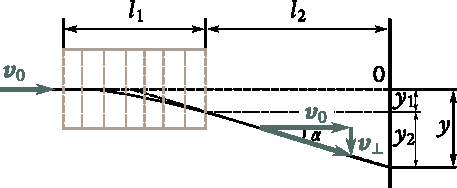
\includegraphics[scale=0.98]{figures/ch_10/fig_10_3.pdf}
		\caption[]{}
		\label{fig:10_3}
	\end{center}
	\vspace{-0.85cm}
\end{figure}

Hạt tích điện sẽ bay theo một đường thẳng theo hướng tạo với vector $\vec{v}_0$ một góc $\alpha$ được xác định theo biểu thức
\begin{equation}\label{eq:10_6}
    \tan\alpha = \frac{v_{\perp}}{v_0} - \frac{e'}{m} E \frac{l_1}{v_0^2}.
\end{equation}

\noindent
Như vậy, chùm tia bị dịch chuyển so với \eqn{10_5} thêm một đoạn
\begin{equation*}
    y_2 = l_2 \tan\alpha = \frac{e'}{m} E \frac{l_1 l_2}{v_0^2},
\end{equation*}

\noindent
với $l_2$ là khoảng cách tới màn từ biên của vùng có trường.

Độ dịch chuyển vết trên màn của tia so với điểm $O$ là 
\begin{equation}\label{eq:10_7}
    y = y_1 + y_2 = \frac{e'}{m} E \frac{l_1}{v_0^2} \parenthesis{\frac{1}{2} l_1 + l_2}.
\end{equation}

\noindent
Thế vào \eqn{10_6}, biểu thức về độ dịch chuyển có thể viết dưới dạng
\begin{equation*}
    y = \parenthesis{\frac{1}{2} l_1 + l_2} \tan\alpha.
\end{equation*}

\noindent
Do đó hạt tích điện bay khi rời vùng có điện trường lệch một góc $\alpha$ đưa ra bởi  \eqn{10_6}.

Giả thiết rằng trên đoạn $l_1$ ta đưa vào một từ trường đều vuông góc với vận tốc $\vec{v}_0$ của các hạt (\fig{10_4}; từ trường vuông góc với mặt phẳng hình vẽ, vùng có trường nằm trong đường tròn gạch).
Do tác dụng của từ trường, mỗi hạt chịu một gia tốc $a_{\perp}=(e'/m)v_0B$ có cường độ không đổi.
Xét giới hạn mà độ lệch của chùm tia bởi từ trường là không lớn, chúng ta có thể coi gia tốc $a_{\perp}$không đổi về cường độ và luôn vuông góc với $v_0$.
Từ đó, chúng ta có thể sử dụng các công thức ở trên để tìm độ dịch chuyển, thế $a_{\perp}=(e'/m)E$ với giá trị $a_{\perp}=(e'/m)v_0B$.
Từ đó, ta nhận được biểu thức cho độ lệch, được ký hiệu là $x$:
\begin{equation}\label{eq:10_8}
    x = \frac{e'}{m} B \frac{l_1}{v_0} \parenthesis{\frac{1}{2} l_1 + l_2}.
\end{equation}

\begin{figure}[t]
	\begin{center}
		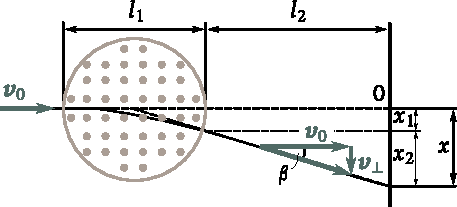
\includegraphics[scale=0.98]{figures/ch_10/fig_10_4.pdf}
		\caption[]{}
		\label{fig:10_4}
	\end{center}
	\vspace{-0.85cm}
\end{figure}

Góc lệch của chùm tia do từ trường được tìm bởi biểu thức
\begin{equation}\label{eq:10_9}
    \tan\beta = \frac{e'}{m} B \frac{l_1}{v_0}.
\end{equation}

\noindent
With a view to \eqn{10_3}, we can write \eqn{10_8} in the form
\begin{equation*}
    x = \parenthesis{\frac{1}{2} l_1 + l_2} \tan\beta.
\end{equation*}

\noindent
Do đó, với các góc lệch nhỏ, hạt rời khỏi từ trường tại góc lệch$\beta$ với độ lớn cho bởi \eqn{10_9}.

Phân tích \eqns{10_7}{10_8} cho thấy độ lệch do từ trường và do điện trường đều tỉ lệ với điện tích riêng của hạt.

Độ lệch của một chùm tia electron bởi từ trường hay điện trường được sử dụng trong các ống cathode.
Một ống làm lệch điện trường (\fig{10_5}), đặt cạnh một súng điện tử tạo ra một chùm các electron tốc độ cao (chùm tia electron), bao gồm 2 cặp tấm làm lệch vuông góc lẫn nhau.
Bằng cách đưa điện áp vào bất kỳ cặp nào, chúng ta có thể tạo ra một độ lệch tương ứng của chùm electron theo phương vuông góc với các tấm làm lệch.
Màn của ống được phủ một lớp huỳnh quang, do đó một điểm sẽ sáng lên trên màn khi chùm electron va vào.

\begin{figure}[t]
	\begin{center}
		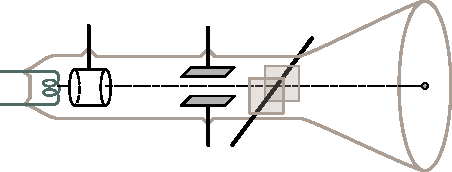
\includegraphics[scale=1]{figures/ch_10/fig_10_5.pdf}
		\caption[]{}
		\label{fig:10_5}
	\end{center}
	\vspace{-0.8cm}
\end{figure}

Ống cathode được dùng trong các dao động ký (oscillograph) - dụng cụ nghiên cứu các quá trình diễn ra nhanh.
Một điện áp thay đổi tuyến tính theo thời gian (điện áp quét) được đưa vào một tấm, và điện áp cần nghiên cứu vào tấm còn lại.
Do khối lượng không đáng kể của một chùm electron, độ lệch của nó gần như ngay lập tức thay đổi theo hiệu điện thế giữa 2 tấm làm lệch và chùm tia sẽ vẽ lên màn của dao động ký một biểu đồ điện thế cần nghiên cứu theo thời gian.
Nhiều đại lượng phi điện tử có thể được chuyển thành tín hiệu điện áp với các dụng cụ thích hợp (bộ chuyển đổi/cảm biến).
Do đó dao động ký được dùng để nghiên cứu đa dạng các quá trình.

Ống cathode là một phần thiết yếu của thiết bị truyền hình.
Trong TV, một ống sử dụng từ trường để điều khiển chùm electron được dùng rộng rãi.
Trong những ống này, các tấm làm lệch được thay thế bằng hai hệ cuộn dây vuông góc lẫn nhau bên ngoài gây ra một từ trường vuông góc với chùm tia.
Thay đổi về dòng trong cuộn kiểm soát chuyển động các điểm sáng tạo nên bởi chùm electron trên màn.

\section{Xác định điện tích và khối lượng
của một electron}\label{sec:10_3}

Điện tích riêng của một electron (\ie, tỉ số $e/m$) đo được lần đầu tiên bởi nhà vật lý người Anh Joseph J. Thomson (1856-1940) vào năm 1897 với dụng cụ là một ống phóng điện \fig{10_6}.
Chùm tia electron (tia cathode; xem \sect{12_6}) phát ra từ một cổng tại anode A đi qua giữa hai tấm của một tụ điện phẳng và va vào một màn huỳnh quang, tạo ra một chấm sáng.
Bằng cách đưa điện áp vào tụ, có thể tạo được một trường điện từ coi như là đều tác dụng lên chùm tia

\begin{figure}[t]
	\begin{center}
		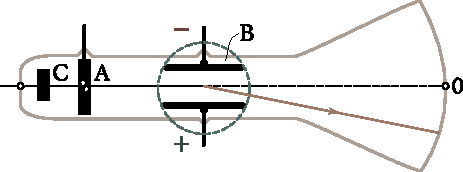
\includegraphics[scale=1]{figures/ch_10/fig_10_6.pdf}
		\caption[]{}
		\label{fig:10_6}
	\end{center}
	\vspace{-0.8cm}
\end{figure}

Ống được đặt giữa hai cực của một nam châm điện, có thể tạo ra một từ trường đều vuông góc với điện trường trên cùng một khoảng trong quỹ đạo của chùm electron (vùng có từ trường được cho trong \fig{10_6} nằm trong đường tròn gạch).
Khi các trường được tắt đi, tia sẽ đập lên màn tại điểm $O$.
Mỗi trường gây ra sự lệch của chùm tia theo phương dụng một cách độc lập.
Độ lớn sự lệch được tính từ \eqns{10_7}{10_8} trong các phần trước.

Sau khi bật từ trường và đo độ lệch của chùm tia
\begin{equation}\label{eq:10_10}
    x = \frac{e}{m} B \frac{l_1}{v_0} \parenthesis{\frac{1}{2} l_1 + l_2},
\end{equation}

\noindent
do từ trường tạo ra, Thomson bật thêm điện trường và tùy chỉnh giá trị sao cho chùm tia sẽ chạm điểm $O$.
Khi này, lực do điện trường và từ trường tác dụng lên chùm electron bằng nhau về độ lớn nhưng ngược chiều.
Điều kiện quan sất được là
\begin{equation}\label{eq:10_11}
    eE = ev_0 B.
\end{equation}

\noindent
Bằng cách giải các phương trình \eqref{eq:10_10} and \eqref{eq:10_11}, Thomson
đã tính được $e/m$ và $v_0$.
H. Busch sử dụng phương pháp hội tụ từ (magnetic focussing) để xác định điện tích riêng của electron.
Phương pháp này được thể hiện sau đây
Xét một chùm tia electron hơi tỏa ra có vận tốc v $v$ đều nhau về độ lớn bay ra từ một điểm trong một từ trường đều.
Chùm tia này đối xứng so với phương của từ trường.
Hướng các electron bay ra tạo một góc nhỏ $\alpha$ với chiều của $\vec{B}$.
Ta tìm được trong \sect{10_1} rằng các electron trong trường hợp này chuyển động theo quỹ đạo xoắn ốc trong một khoảng thời gian như nhau
\begin{equation*}
    T = 2\pi \frac{m}{e} \frac{1}{B},
\end{equation*}

\noindent
thực hiện được một vòng quay và dịch chuyển dọc hướng của trường một đoạn $l$ bằng
\begin{equation}\label{eq:10_12}
    l = v\cos\alpha \times T.
\end{equation}

\noindent
Do góc $\alpha$ khá nhỏ, chiều dài \eqref{eq:10_12} với các electron khác nhau có cùng $vT$ hầu như là bằng nhau (với các góc nhỏ $\cos\alpha\approx 1$).
Do đó, chùm tia hơi mở này sẽ hội tụ tại một điểm cách điểm phát electron một đoan
\begin{equation}\label{eq:10_13}
    l = vT = 2 \pi \frac{m}{e} \frac{v}{B}
\end{equation}

\noindent

\begin{figure}[t]
	\begin{center}
		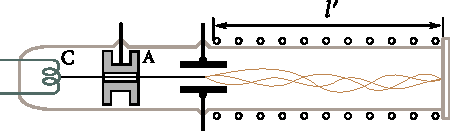
\includegraphics[scale=1]{figures/ch_10/fig_10_7.pdf}
		\caption[]{}
		\label{fig:10_7}
	\end{center}
	\vspace{-0.8cm}
\end{figure}

Trong thí nghiệm của Busch (\fig{10_7}) được gia tốc khi đi qua hiệu điện thế $U$ giữa cathode và anode A.
Từ đó, chúng nhận được vận tốc $v$ có thể tìm được từ liên hệ
\begin{equation}\label{eq:10_14}
    eU = \frac{mv^2}{2}.
\end{equation}

\noindent
Sau khi thoát khỏi một cổng trên anode, các electron này tạo ra một chùm tia hẹp hướng dọc theo chiều của một ống chân không được đưa vào trong một cuộn dây (solenoid).
Một tụ điện được cấp điện thế biến đổi được đưa vào lõi cuộn 
Điện trường do tụ gây ra làm chệch hướng các electron trong tia khỏi trục của cuộn dây một góc nhỏ $\alpha$ biến đổi theo thời gian.
Điều này dẫn tới sự ``xoáy'' của chùm tia --- các electron bắt đầu chuyển động theo các quỹ đạo xoắn ốc khác nhau.
Một màn huỳnh quang được đặt tại đầu ra của cuộn dây.
Nếu cảm ứng từ $B$ được chọn sao cho khoảng cách $l'$ từ tụ đến màn thỏa mãn yêu cầu
\begin{equation}\label{eq:10_15}
    l' = n l
\end{equation}

\noindent
($l$ là bước của đường xoắn ốc và $n$ là một số nguyên dương), thì giao điểm của các quỹ đạo electron va vào màn được hội tụ vào một điểm và sinh ra một điiểm sáng rõ trên màn.
Nếu điều kiện \eqref{eq:10_15} không đạt được, điểm sáng trên màn sẽ bị nhòe đi.
Ta có thể tìm $e/m$ and $v$ bằng cách giải hệ phương trình \eqref{eq:10_13}, \eqref{eq:10_14}, và
\eqref{eq:10_15}.

Kết quả chính xác nhất của điện tích riêng electron được đưa ra với xem xét kết quả của nhiều phương pháp, là
\begin{equation}\label{eq:10_16}
    \frac{e}{m} = \SI{1.76e11}{\coulomb\per\kilo\gram} = \num{5.27e17} \cgs{e}{q}\,\si{\per\gram}.
\end{equation}

\begin{figure}[t]
	\begin{center}
		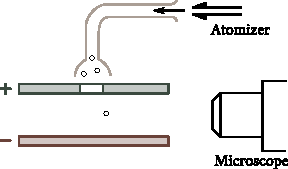
\includegraphics[scale=1]{figures/ch_10/fig_10_8.pdf}
		\caption[]{}
		\label{fig:10_8}
	\end{center}
	\vspace{-0.8cm}
\end{figure}

Phương trình \eqref{eq:10_16} cho tỉ số giữa điện tích electron và khối lượng nghỉ $m$.
Trong thí nghiệm thực hiện bởi Thomson, Busch và trong các thí nghiệm tương tự, người ta đo được tỉ số giữa điện tích và khối lượng tương đối tính.
\begin{equation}\label{eq:10_17}
    \ab{m}{r} = \frac{m}{\sqrt{1 - \parenthesis{v^2/c^2}}},
\end{equation}

\noindent
Trong thí nghiệm của Thomson, tốc độ electron vào khoảng $0.1c$.
Tại tốc độ này, khối lượng tương đối tính cao hơn khối lượng nghỉ khoảng $0.5\%$.
Trong các thí nghiệm sau đó, tốc độ của electron đạt tới rất cao.
Trong tất cả trường hợp, người làm thưc nghiệm đều phát hiện sự giảm của $e/m$ với sự tăng của $v$, đều diễn ra theo \eqn{10_17}.

Điện tích của một electron được xác định với độ chính xac cao bởi nhà khoa học Mỹ Robert Milikan (1886-1953) vào năm 1909.
Ông đưa các giọt dầu cực nhỏ vào khoảng không giản giữa 2 bản tụ nằm ngang(\fig{10_8}).
Khi dầu được tách thành giọt, các giọt này được tích điện và có thể lơ lửng trên không khi chọn đúng độ lớn và chiều của điện thế của tụ.
Điều kiện cân bằng là
\begin{equation}\label{eq:10_18}
    P' = e' E.
\end{equation}

\noindent
Ở đây $e'$ là điện tích của một giọt và $P'$ và hợp lực của lực đẩy và trọng lực
\begin{equation}\label{eq:10_19}
    P' = \frac{4}{3} \pi r^2 (\rho - \rho_0) g
\end{equation}

\noindent
($\rho$ là mật độ của giọt, $r$ là bán kính và $\rho_0$ là mật độ không khí).

Phương trình \eqref{eq:10_18} và \eqref{eq:10_19} can thể sử dụng để tìm $e$ nếu ta biết$r$.
Để tìm bán kính, tốc độ rơi đều $v_0$ của một giọt được đo trong điều kiện không có từ trường
Chuyển động đều của giọt cho thấy rằng lực $P'$ được cân bằng bởi lực cản $F = 6\pi\eta rv$ [xem Pt. (9.24) cuốn I; $\eta$ là độ nhớt không khí]:
\begin{equation}\label{eq:10_20}
    P' = 6 \pi \eta r v_0.
\end{equation}

\noindent
Chuyển động của một giọt được quan sát với sự trợ giúp của một kính hiển vi
Để đo $v_0$, người ta đo thời gian giọt này chuyển động giữa 2 sợi mảnh soi được bởi kính hiển vi.

Việc giữ một giọt chất lỏng lơ lửng một cách chính xác gần như bất khả thi
Do đó, thay vì chọn một điện trường phù hợp với điều kiện \eqref{eq:10_18}, một điện trường được bật lên mà theo đó giọt dầu này bắt đầu chuyển động hướng lên với một tốc độ nhỏ
Vận tốc hướng lên đều $v_E$ được xác định từ điều kiện rằng lực $P'$ và lực$6\pi\eta rv$ cân bằng với lực $e'E$:
\begin{equation}\label{eq:10_21}
    P' + 6\pi\eta rv_E = e'E.
\end{equation}

Khử $P'$ và $r$ từ Eqs. \eqref{eq:10_19}, \eqref{eq:10_20}, and \eqref{eq:10_21}, ta có biểu thức cho $e'$:
\begin{equation}\label{eq:10_22}
    e' = 9\pi \bracket{ \frac{2\eta^3 v_0}{(\rho-\rho_0)g} }^{1/2} \parenthesis{ \frac{v_0+v_E}{E} }
\end{equation}

\noindent
(Millikan đưa ra một chỉnh sửa cho phương trình này khi tính đến việc độ lớn của giọt dầu có thể so sánh với chiều dài tự do trung bình của phân tử không khí).

Do đó bằng cách đo tốc độ rơi tự do của giọt dầu $v_0$ và tốc độ đi lên $v_E$ trong một điện trường xác định $E$, ta có thể xác định điện tích của giọt dầu $e'$.
Khi đo tốc độ $v_E$ tại các giá trị nào đó của $e'$, Millikan ion hóa không khí bằng cách chiếu tia X qua không gian giữa hai bản tụ.
Các ion khác nhau dính vào giọt dầu và làm thay đổi điện tích của nó.
Từ đó tốc độ $v_E$ thay đổi theo.
Sau khi đo giá trị tốc độ mới, không gian giữa hai bản tụ tiếp tục được chiếu xạ, và cứ thế tiếp diễn.

Thay đổi về điện tích của giọt $\Delta{e'}$ và chính điện tích $e'$ được đo bởi Millikan sau mỗi lần đều được xác định là một số nguyên lần của một đai lượng $e$.
Đây là bằng chứng thực nghiệm về bản chất rời rạc của điện tích, \ie, việc tất cả điện tích đều chứa các điện tích cơ bản có cùng độ lớn

Giá trị của điện tích cơ bản được thiết lập dựa theo đo đạc của Millikan và các dữ liệu thu được bằng các phương pháp khác là
\begin{equation}\label{eq:10_23}
    e = \SI{1.60e-19}{\coulomb} = \SI{4.80e-10} {\cgs{e}{q}}.
\end{equation}

\noindent
Điện tích của một electron có cùng giá trị

Khối lượng nghỉ của một electrong đo được từ \eqns{10_16}{10_23} là
\begin{equation}\label{eq:10_24}
    m = \SI{0.91e-30}{\kilo\gram} = \SI{0.91e-23} {\gram}.
\end{equation}

\noindent
Giá trị này vào khoảng $1/1840$ khối lượng của hạt nhân nguyên tử nhẹ nhất-hạt nhân hydro.

Các định luật điện phân được thiết lập bằng thực nghiệm bởi Michael Faraday vào năm 1836 đóng vai trò lớn trong việc phát hiện bản chất rời rạc của điện tích.
Theo các định luật này, khối lượng $m$ của một chất
được giải phóng khi một dòng điện đi qua một chất điện li\footnote{Chất điện li là hỗn hợp của muối, kiềm hoặc acid trong nước và một số chất lỏng khác và đồng thời các muối tan ở trạng thái tinh thể ion ở thể rắn. Các biến đổi hóa học diễn ra trong chất điện li khi có dòng điện đi qua. Các chất này được gọi là vật dẫn điện li(electrolytic conductior) (vật dẫn loại hai) để phân biệt khỏi vật dẫn điện tử (electronic conductor) (vật dẫn loại một) khi mà dòng điện đi qua không đi kèm phản ứng hóa học} tỉ lệ thuận với điện tích $q$truyền đi bởi dòng điện:
\begin{equation}\label{eq:10_25}
    m = \frac{1}{F} \frac{M}{z} q.
\end{equation}

\noindent
Tại đây $M$ là khối lượng một mol chất được giải phóng, $z$ là hóa trị của chất này và $F$ là \textbf{hằng số Faraday} (\textbf{số Faraday}) có giá trị bằng
\begin{equation}\label{eq:10_26}
    F = \SI{96.5e3}{\coulomb\per\mole}.
\end{equation}

Chia hai vế của \eqn{10_25} cho khối lượng của một ion, ta có
\begin{equation*}
    N = \frac{1}{F} \frac{\ab{N}{A}}{z} q,
\end{equation*}

\noindent
với $\ab{N}{A}$ là hằng số Avogadro và $N$ là số lượng ion trong khối lượng $m$.

Từ đó điện tích của một ion
\begin{equation*}
    e' = \frac{q}{N} = \frac{F}{\ab{N}{A}} z.
\end{equation*}

\noindent
Do đó, điện tích của một ion là một số nguyên lần của đại lượng
\begin{equation}\label{eq:10_27}
    e = \frac{F}{\ab{N}{A}},
\end{equation}

\noindent
chính là điện tích cơ bản.

Từ đó, bản chất rời rạc của điện tích được thể hiện bởi ion trong các chất điện li có thể được suy ra từ phân tích các định luật điện phân.

Thế $F$ cho \eqn{10_27} giá trị từ \eqn{10_26} và cho $\ab{N}{A}$ giá trị từ thí nghiệm của J.Perrin (xem phần 11.9 của tập I), ta tìm được giá trị tương đối khớp với giá trị tìm được bởi Millikan.

Do độ chính xác của hằng số Faraday và độ chính xác của giá trị $e$ thu được bởi Millikan lớn hơn rất nhiều so với độ chính xác của thí nghiệm Perrin dùng để tìm $\ab{N}{A}$, \eqn{10_27} được sử dụng để xác định hằng số Avogadro.
Ở đây, $F$ được tìm từ thực nghiệm với điện phân và giá trị của $e$ thu được bởi Millikan được sử dụng

\section{Xác định điện tích riêng của Ion. Khối phổ kế(Mass spectrograph)}\label{sec:10_4}

Phương pháp xác định điện tích riêng đưa ra tại các phần trước phù hợp khi tất cả các hạt trong một chùm tia có cùng vận tốc.
Tất cả electron cấu thành chùm tia được gia tốc bởi cùng một hiệu điện thế đưa vào giữa cathode mà electron bay ra và anode.
Do đó, độ loe giá trị vận tốc của electron trong một chùm tia là rất nhỏ.
Nếu không có điều này, một chùm tia electron sẽ tạo thành một điểm nhòe trên màn và không thể đo đạc được

Ion được hình thành do sự ion-hóa các phân tử của một chất khí diễn ra tại phần thể tích có kích thước đáng kể.
Xuất hiện tại các phần khác nhau của khối khí này, các ion di chuyển qua các hiệu điện thế khác nhau, và do đó, vận tốc của chúng sẽ khác nhau.
Từ đó, phương pháp được dùng để đo điện tích riêng của electron không thể được áp dụng cho ion.
Trong năm 1907, J.J. Thomson phát triển ``phương pháp parabol'', cho phép khắc phục được khó khăn nêu trên.

\begin{figure}[t]
	\begin{center}
		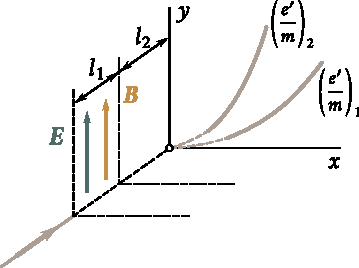
\includegraphics[scale=1]{figures/ch_10/fig_10_9.pdf}
		\caption[]{}
		\label{fig:10_9}
	\end{center}
	\vspace{-0.8cm}
\end{figure}

Trong thí nghiệm của Thomson, một chùm tia ion dương hẹp xuyên qua một vùng có tác động đồng thời của điện trường và từ trường song song (\fig{10_9}).
Cả hai trường có thể coi là đều và vuông góc với phương ban đầu của chùm tia.
Chúng làm chệch quỹ đạo của các ion: từ trường làm chệch theo phương của trục $x$, điện trường dọc theo trục $y$.
Theo \eqns{10_8}{10_7}, độ lệch này là
\begin{equation}\label{eq:10_28}
    \begin{split}
        x &= \frac{e'}{m} B \frac{l_1}{v} \parenthesis{\frac{1}{2} l_1 + l_2}\\
        y &= \frac{e'}{m} E \frac{l_1}{v^2} \parenthesis{\frac{1}{2} l_1 + l_2},
    \end{split}
\end{equation}

\noindent
với $v$ là vận tốc của một ion nào đó với điện tích riêng $e'/m$, $l_1$ là chiều dài vùng mà các trường tác động lên chùm tia và $l_2$ là khoảng cách từ biên của vùng trên tới tấm phim dùng để ghi các ion đập vào.

Các công thức \eqref{eq:10_28} là tọa độ của điểm mà một ion có giá trị $e'/m$ cho trước và vận tốc $v$ đập lên phim.
Các ion có cùng điện tích riêng, nhưng vận tốc khác nhau, đập vào các điểm khác nhau trên phim.
Khử vận tốc $v$ từ pt. \eqref{eq:10_28}, ta có phương trình đường chứa vết các ion có cùng giá trị $e'/m$:
\begin{equation}\label{eq:10_29}
    y = \frac{E}{B^2 l_1 (0.5 l_1 + l_2)} \frac{m}{e'} x^2.
\end{equation}

Phân tích \eqn{10_29} cho thấy các ion có cùng giá trị $e'/m$ và các giá trị khác nhau của $v$ để lại vệt có dạng parabol trên phim.
Ion có các giá trị $e'/m$ khác tương ứng với các parabol khác nhau.
Phương trình \eqref{eq:10_29} có thể dùng để tìm điện tích riêng của ion ứng với mỗi parabol nếu các tham số của dụng cụ đã biết (\ie, $E$, $B$, $l_1$, and $l_2$), và độ lệch $x$ và $y$ được đo.
Khi chiều của một trường được đảo lại, tọa độ liên quan bị đảo dấu và đưa đến các parabol đối xứng với ban đầu.
Chia đôi khoảng cách giữa các điểm tương ứng trên các parabol đối xứng này giúp tìm được $x$ và $y$.
Vệt để lại trên phim khi các trường được tắt cho biết gốc tọa độ. Hình \ref{fig:10_10} cho thấy parabol đầu tiên thu được bởi Thomson.

\begin{figure}[t]
	\begin{center}
		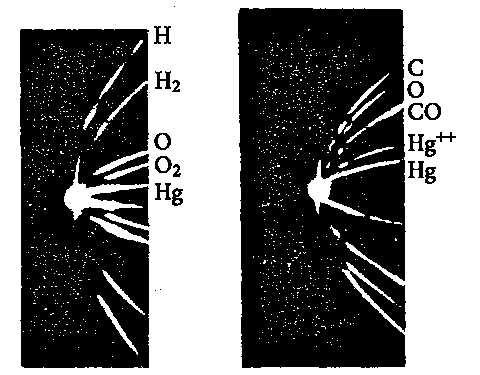
\includegraphics[scale=0.9]{figures/ch_10/fig_10_10.pdf}
		\caption[]{}
		\label{fig:10_10}
	\end{center}
	\vspace{-0.8cm}
\end{figure}

Khi thí nghiệm với khí neon tinh khiết, Thomson phát hiện rằng khí này vẽ ra hai parabol tương ứng với khối lượng hạt nhân tương đối $20$ và $22$.
Kết quả này đưa đến giả thiết rằng có hai biến thể của nguyên tử neon không thể phân biệt bằng phương pháp hóa học (ngày nay ta gọi chúng là \textbf{đồng vị} của neon).
This assumption was proved by the British scientist Francis Aston (1877-1945), who improved the method of determining the specific charge of ions.
Giả thiết này được chứng minh bởi nhà khoa học Anh Francis Aston (1877-1945), người cải thiện phương pháp xác định điện tích riêng của ion.
\begin{figure}[t]
	\begin{center}
		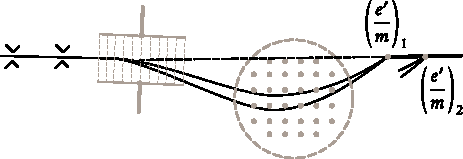
\includegraphics[scale=1]{figures/ch_10/fig_10_11.pdf}
		\caption[]{}
		\label{fig:10_11}
	\end{center}
	\vspace{-0.75cm}
\end{figure}

Dụng cụ của Aston, được ông gọi là \textbf{khối phổ kế} (mass spectrograph), được thiết kế như sau (\fig{10_11}).
Một chùm ion được tách ra bởi các khe xuyên qua một từ trường và điện trường.
Những trường này được định hướng sao cho các ion chuyển động tới các phía khác nhau.
Khi chúng đi qua điện trường, các ion với giá trị $e'/m$ cho trước bị lệch nhiều khi vận tốc thấp hơn.
Do đó, các ion rời điện trường dưới dạng một chùm tia tỏa ra.
Quxy đạo của các ion cũng được bẻ cong nhiều hơn trong từ trường khi vận tốc thấp hơn.
Do các ion bị lệch về hai phía bởi hai trường, sau khi rời từ trường chúng tạo thành một chùm tia hội tụ tại một điểm.

\begin{figure}[t]
	\begin{center}
		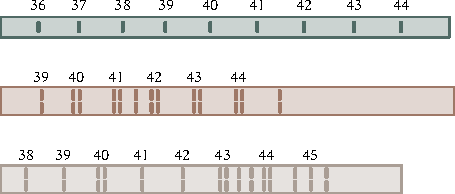
\includegraphics[scale=0.93]{figures/ch_10/fig_10_12.pdf}
		\caption[]{}
		\label{fig:10_12}
	\end{center}
	\vspace{-0.9cm}
\end{figure}

Các ion với giá trị điện tích riêng khác được hội tụ tại các điểm khác (quỹ đạo của các ion với một giá trị $e'/m$ được cho trong \fig{10_11}).
Các tính toán cho thấy các điểm hội tụ của các chùm ion có các giá trị $e'/m$ khác nhau gần như nằm trên một đường thẳng (đường gạch trong hình).
Đặt một tấm phim dọc theo đường này, Aston thu được một số đường thẳng trên nó, mỗi đường ứng với một giá trị của $e'/m$.
Sự tương tự của ảnh trên phim với ảnh một dải quang phổ là lý do Aston gọi nó là khối phổ (mass spectrogram), và dụng cụ thí nghiệm này - khối phổ kế (mass spectrograph).
Hình \ref{fig:10_12} cho thấy dải khối phổ thu được bởi Aston (số khối của các ion tương ứng được chỉ ra tương ứng với đường).

K. Bainbridge thiết kế một dụng cụ theo hướng khác
Trong khối phổ kế Bainbridge (\fig{10_13}), một chùm ion đi qua bộ lọc vận tốc, tách cácác ion có vận tốc khác nhau khỏi chùm.
Trong bộ lọc này, các ion chịu tác dụng của điện trường và từ trường vuông góc làm lệch các ion đến các phía khác nhau.
Chỉ các ion có tác dụng của điện trường và từ trường bù trừ lẫn nnhau vượt qua được khe lọc.
Điều kiện này là $e'E = e'vB$.
Do đó vận tốc của các ion rời bộ lọc không phụ thuộc vào khối lượng hay vận tốc có giá trị như nhau bằng $v = E/B$.

\begin{figure}[t]
	\begin{center}
		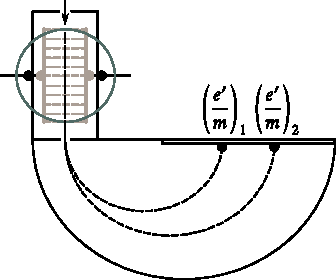
\includegraphics[scale=1]{figures/ch_10/fig_10_13.pdf}
		\caption[]{}
		\label{fig:10_13}
	\end{center}
	\vspace{-0.8cm}
\end{figure}

Sau khi rời bộ lọc, các ion đi vào vùng từ trường đều có giá trị $B'$ vuông góc với vận tốc.
Trong vùng này, chúng di chuyển dọc đường tròn có bán kính phụ thuộc vào $e'/m$:
\begin{equation*}
    R = \frac{m}{e'}\frac{v}{B'}
\end{equation*}

[see \eqn{10_21}].

Sau khi đi được một nửa đường tròn, các ion đập vào tấm phim tại khoảng cách $2R$ tính từ khe lọc.
Do đó, ion của từng loại (xác định bởi giá trị $e'/m$) để một vết trên phim dưới dạng một vạch nhỏ.
Điện tích riêng của ion có thể được tính khi tham số của dụng cụ đã được biết.
Do điện tích của các ion là một số nguyên lần điện tích cơ bản $e$, khổi lượng ion có thể được tính từ giá trị đã biết $e'/m$.

Hiện tại, người ta sử dụng đa dạng loại khối phổ kế.
Các dụng cụ cũng thiết kế để ghi nhận ion bằng thiết bị điện tử thay vì một tấm phim.
Chúng được gọi là \textbf{máy khối phổ (mass spectrometer)}.

\section{Gia tốc của hạt tích điện}\label{sec:10_5}

Các thí nghiệm sử dụng chùm hạt tích điện năng lượng cao có vai trò quan trọng trong vật lý hạt nhân và hạt cơ bản.
Các thiết bị được sử dụng để tạo ra các chùm hạt như thế được gọi là \textbf{Máy gia tốc hạt}.
Có nhiều loại thiết bị như thế.
Chúng ta sẽ làm quen với nguyên lý hoạt động của một số trong đó.

\begin{figure}[t]
	\begin{center}
		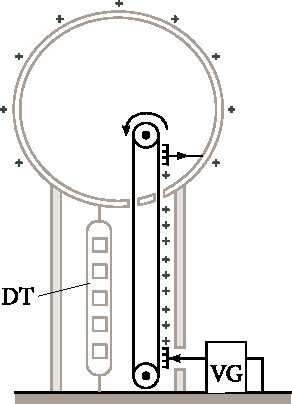
\includegraphics[scale=1]{figures/ch_10/fig_10_14.pdf}
		\caption[]{}
		\label{fig:10_14}
	\end{center}
	\vspace{-0.8cm}
\end{figure}

\textbf{Máy phát Van De Graaff}. Trong năm 1929, R. van de Graaff thiết kế một máy phát tĩnh điện dựa trên nguyên lý rằng điện tích dư sẽ có vị trí nằm trên mặt ngoài của vật dẫn.
Sơ đồ của máy phát được cho trong\fig{10_14}.
Một khối cầu rỗng bằng kim loại để làm vật dẫn được đặt trên một trụ cách điện
Một đai bằng lụa hoặc sợi cao su di chuyển liên tục gắn trên trục được đưa lại khối cầu
Một chuỗi các kim nhọn có dạng cái lược được đặt tại gốc của cột gần đai này.
Các điện tích sinh ra bởi một máy phát điện thế (voltage generator-VG) với vài kilovolt chạy vào đai từ các điểm kim nhọn.
Vật dẫn chứa một chuỗi kim nhọn thứ hai để các điện tích chạy vào từ đai.
Chuỗi kim này được nối tới vật dẫn như hình \fig{10_14} sao cho điện tích chạy khỏi đai ngay lập tức truyền đến mặt ngoài.
Khi điện tích tự lại trên vật dẫn, điện thế vật dẫn tăng lên cho đến khi lượng điện tích rò ra ngoài bằng lượng điện tích được đưa đến
Sự rò rỉ này đa phần do sự ion hóa không khí gần bề mặt điện tích
Dòng điện chạy qua không khí được gọi là phóng điện hình vương miện (corona discharge) (xem phần \sect{12_8}).
Bề mặt vật dẫn được mài cẩn thận để giảm thiểu sự phóng điện này.


Điện thế mà vật dẫn có thể phóng điện được giới hạn bởi điều kiện rằng tại điện trường khoảng \SI{3}{\kilo\volt\per\metre}
(\SI{30}{\kilo\volt\per\centi\metre}) sẽ có hiện tượng phóng điện trong không khí tại áp suất khí quyển
Với một hình cầu,  $E=\varphi/r$.
Do đó, để đạt được hiệu điện thế cao hơn, độ lớn của vật dẫn cũng phải tăng(có thể lên tới đường kính \SI{10}{\metre}).
Hiệu điện thế lớn nhất có thể thu được trên thức tế với một máy phát van de Graaff là khoảng \SI{10}{\mega\volt} (\SI{e7}{\volt}).

Các hạt được gia tốc trong một ống phóng điện mà hiệu điện thế của các điện cực được lấy từ máy phát. 
Một máy phát van de Graaff cocó thể được thiết kế thành 2 trụ tương đương đặt gần nhau với phần vật dẫn được tích điện trái dấu.
Trong trường hợp này, ống phóng điện được nối giữa các vật phẫn

Chú ý rằng đai phát điện, vật dẫn, ống phóng và đất phải được nối thành một mạch kín.
Trong ống phóng, các điện tích di chuyển do tác động của lực tĩnh điện.
Điện tích được đưa từ đất vào vật dãn bởi các lực ngoại li với một phần là lực cơ học khiến đai phát điện chuyển động.
\begin{figure}[t]
	\begin{center}
		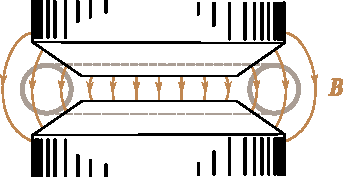
\includegraphics[scale=1]{figures/ch_10/fig_10_15.pdf}
		\caption[]{}
		\label{fig:10_15}
	\end{center}
	\vspace{-0.8cm}
\end{figure}

\textbf{Betatron.} Đây là tên được đặt cho máy gia tốc cảm ứng electron sử dụng điện trường xoáy
Nó bao gồm một buồng chân không hình xuyến được đặt giữa các cực của một nam châm điện có hình dạng đặc biệt (\fig{10_15}).
Cuộn dây của nam châm được tiếp một dòng điện xoay chiều có tần số khoảng \SI{100}{\hertz}.
Từ trường biến thiên này có hai chức năng: thứ nhất, nó tạo ra một điện trường xoáy giúp tăng tốc các electron, và thứ hai, nó giữ các electron trong một quỹ đạo trùng với trục của hình xuyến

Để giữ các electron này trong một quỹ đạo với bán kính không đổi, từ trường phải được tăng khi vân tốc tăng [theo \eqn{10_2},bán kính quỹ đạo tỉ lệ thuận với $v/B$].
Do đó, chỉ có ở các kỳ thứ hai và thứ tư của một chu kỳ có thể được dùng để gia tốc vì tại thời điểm đầu của các kỳ này, dòng điện trong nam châm điện bằng không.
Do đó một betatron hoạt động theo nhịp
Tại thời điểm đầu của nhịp, một súng electron bắn một chùm electron vào hình xuyến.
Chùm tia này cắt qua điện trường xoáy và bắt đầu chuyển động theo một quỹ đạo tròn với vận tốc tăng dần đều.
Trong kỳ tăng của từ trường (khoảng \SI{e-3}{\second}), các electron có thể hoàn thành hàng triệu vòng xoay và nhận được năng lượng khoảng vài trăm \si{\mega\electronvolt}.
Với năng lượng lớn thế này, tốc độ của electron đạt tới xấp xỉ tốc độ ánh sáng $c$.

Để một electron được tăng tốc chuyển động trong một quỹ đạo tròn bán kính $r_0$, một liên hệ đơn giản mà ta sẽ suy ra sau đây phải đạt được giữa điện trường tại quỹ đạo và bên trong nó.
Điện trường xoáy này được hướng dọc tiếp tuyến quỹ đạo mà electron đang di chuyển
Do đó, lưu số của vector $\vec{E}$ dọc quỹ đạo này là $2\pi r_0E$.
Khi đó theo công thức \eqn{9_19}, lưu số của vector $\vec{E}$ là $-(\diffin{\Phi}{t})$, với $\Phi$ là từ thông qua mặt bao bởi quỹ đạo
Dấu trừ thể hiện chiều của $\vec{E}$.
Ở đây ta chỉ quan tâm tới độ lớn của trường, do đó ta sẽ bỏ qua dấu trừ này.
Thế vào công thức cho lưu số, ta được
\begin{equation*}
    E = \frac{1}{2\pi r_0} \diff{\Phi}{t}.
\end{equation*}

\noindent
Từ trường vuông góc với mặt phẳng chuyển động.
Do đó có thể giả thiết rằng $\Phi=\pi r^2_0\average{B}$, với $\average{B}$ là giá trị trung bình của cường độ cảm ứng từ.
Do đó,
\begin{equation}\label{eq:10_30}
    E = \frac{1}{2\pi r_0} \diff{}{t} \parenthesis{ \pi r^2_0 \average{B}} = \frac{r_0}{2} \diff{}{t} \average{B}.
\end{equation}

Phương trình chuyển động tương đối tính của electron trên quỹ đạo:
\begin{equation}\label{eq:10_31}
    \diff{}{t}\bracket{ \frac{m \vec{v}}{\sqrt{1-\parenthesis{v^2/c^2}}} } = e \vec{E} + e \vec{v} \times \ab{\vec{B}}{orb}
\end{equation}

\noindent
($\ab{\vec{B}}{orb}$ là cường độ cảm ứng từ trên quỹ đạo).

Vận tốc của một electron chuyển động dọc một đường tròn bán kính $r_0$ có thể viết dưới dạng $\vec{v}=\omega r_0 \hatvec{\tau}$, với $\omega$ là vận tốc góc của electron và  $\hatvec{\tau}$ vector đơn vị tiếp tuyến với quỹ đạo.
Vector $\vec{E}$ có thể được viết dưới dạng 
\begin{equation*}
    \vec{E} = E \hatvec{\tau} = \frac{r_0}{2} \diff{}{t} \average{B} \hatvec{\tau}
\end{equation*}

\noindent
[xem \eqn{10_30}].
Cuối cùng, tích $\vecprod{v}{B}$ có thể viết dưới dạng $vB\hatvec{n}=\omega r_0 B\hatvec{n}$, với $\hatvec{n}$ là vector đơn vị pháp tuyến với quỹ đạo.
Thế những điều được đưa ra ở trên, có thể viết \eqn{10_31} dưới dạng:
\begin{equation}\label{eq:10_32}
    \diff{}{t}\bracket{ \frac{\omega r_0 \hatvec{\tau}}{\sqrt{1 - \parenthesis{\omega^2r_0^2/c^2}}} } = \frac{er_0}{2} \diff{}{t} \average{B} \hatvec{\tau} + e\omega r_0 \ab{B}{orb} \hatvec{n}.
\end{equation}

Đạo hàm theo thời gian của vector đơn vị $\hatvec{\tau}$ là $\hatvec{\tau}=\omega\hatvec{n}$ [xem Eq. (1.56) tại Tập I; vận tốc góc chuyển động quay của vector đơn vị $\hatvec{\tau}$ bằng vận tốc góc của electron].
Do đó, lấy đạo hàm ở vế trái của \eqn{10_32}, ta có công thức
\begin{equation*}
    \diff{}{t}\bracket{ \frac{\omega r_0}{\sqrt{1 - \parenthesis{\omega^2r_0^2/c^2}}} } \hatvec{\tau} + \bracket{ \frac{\omega r_0}{\sqrt{1 - \parenthesis{\omega^2r_0^2/c^2}}} } \omega \hatvec{n} = \frac{e r_0}{2} \diff{}{t} \average{B} \hatvec{\tau} + e \omega r_0 \ab{B}{orb} \hatvec{n}.
\end{equation*}

\noindent
Quy đồng thừa số của các vector đơn vị tương ứng ở vế trái và vế phải của phương trình, ta có
\begin{align}
    \diff{}{t}\bracket{ \frac{\omega r_0}{\sqrt{1 - \parenthesis{\omega^2r_0^2/c^2}}} } &= \frac{e r_0}{2} \diff{}{t} \average{B}, \label{eq:10_33}\\
    \frac{\omega r_0}{\sqrt{1 - \parenthesis{\omega^2r_0^2/c^2}}} &= er_0 \ab{B}{orb}. \label{eq:10_34}
\end{align}

\noindent
Từ \eqn{10_33} suy ra
\begin{equation}\label{eq:10_35}
    \frac{\omega r_0}{\sqrt{1 - \parenthesis{\omega^2r_0^2/c^2}}} = \frac{e r_0}{2} \average{B}
\end{equation}

\noindent
($\omega$ và $\average{B}$ tại khỏi đầu của một nhịp bằng 0.)

So sánh \eqns{10_34}{10_35} cho thấy:
\begin{equation*}
    \ab{B}{orb} = \frac{1}{2} \average{B}.
\end{equation*}

\noindent
Do đó, để một electron chuyển động liên tục trong một quỹ đạo tròn, cảm ứng từ trên quỹ đạo phải bằng một nửa giá trị trung bình của cảm ứng từ bên trong quỹ đạo.
Ta có thể đạt điều này bằng cách mài các trụ thành hình nón cụt  (như \fig{10_15}).

Tại thời điểm cuối một kỳ gia tốc, một từ trường được bật lên thêm để đẩy electron khỏi quỹ đạo cân bằng và hướng về một bia đặc biệt bên trong hình xuyến.
Khi đập vào bia, electron phát ra bức xạ điện từ năng lượng cao (tia gamma, tia X).

Betatron được sủ dụng chủ yếu cho pháp lý hạt nhân. Các máy gia tốc nhỏ đạt đến nawg lượng \SI{50}{\mega\electronvolt} được sử dụng trong công nghiệp làm nguồn cho các tia X rất mạnh để phát hiện các lỗi trong vật liệu.

\textbf{Cyclotron.} Máy gia tốc này được đưa trên nguyên lý rằng chu kỳ chuyển động của một hạt tích điện trong một từ trường đều không phụ thuộc vào vận tốc [xem  \eqn{10_3}].
Thiết bị này gồm hai điện cực dưới dạng nửa một hộp trụ tròn thấp (\fig{10_16}\footnote{Hình này được lấy từ \texttt{https://commons.wikimedia.org/wiki/File:Zyclotron.svg}.}) gọi là dee.
Các dee được đặt trong một vùng chân không đặt giữa hai cực của một nam châm điện lớn.
Từ trường sinh ra bởi nam châm là đều và vuông góc với mặt phẳng của dee.
Các dee được được cung cấp một điện áp xoay chiều từ một máy phát điện cao tần.

\begin{figure}[t]
	\begin{center}
		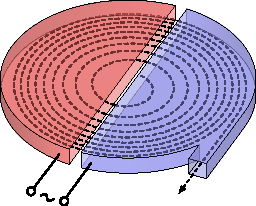
\includegraphics[scale=1]{figures/ch_10/fig_10_16.pdf}
		\caption[]{}
		\label{fig:10_16}
	\end{center}
	\vspace{-0.8cm}
\end{figure}

Ta đưa một hạt tích điện vào khe giữa hai dee vào thời điểm điện tích đạt giá trị lớn nhất
Hạt này sẽ bị kéo vào một dee dưới tác động của điện trường.
Không gian bên trong dee là đẳng thế, do đó hạt chỉ chuyển động dưới tác động của từ trường
Trong tường hợp này, hạt chuyện động trong một đường tròn với bán kính tỉ lệ thuận với vận tốc [xem \eqn{10_2}].
Ta chọn tần số điện áp giữa các dee sao cho tại thời điểm mà hạt tiếp cận khe giữa hai dee sau khi chuyển động một nửa đường tròn, hiệu điện thế giữa hai dee sẽ đảo dấu và đạt giá trị cực đại (của biên độ).
Bây giờ hạt sẽ được gia tốc lần nữa và bay vào dee thứ hai với năng lượng gấp đôi lần chuyển động trong dee thứ nhất.
Với vận tốc lớn hơn, hạt sẽ chuyển động theo một đường tròn với bán kính lớn hơn ($R$ tỉ lệ thuận với $v$), nhưng thời gian di chuyển sẽ giữ nguyên.
Do đó, tại thời điểm hạt tới khe giữa hai dee, điện áp giữa chúng sẽ đổi dấu lần nữa vào đạt giá trị cực đại.

Do đó hạt chuyển động theo một đường cong gần giống một đường xoắn ốc, và mỗi lần đi qua khe giữa hai dee nó nhận được thêm một phần năng lượng bằng $e'\ab{U}{m}$ ($e'$ là điện tích của hạt, and $\ab{U}{m}$ là biên độ của điện áp do máy phát).
Với một nguồn xoay chiều tương đối nhỏ ($\ab{U}{m}$ khoảng \SI{e5}{\volt}) ta có thể dùng cyclotron để gia tốc proton tới năng lượng khoảng \SI{25}{\mega\electronvolt}.
Tại mức năng lượng cao hơn [theo \eqn{10_3} thì bán kính tỉ lệ thuận với $m$ (khối lượng tương đối tính - ND)], và sự đồng bộ giữa chuyển động của hạt và biến thiên điện trường bị vi phạm.

Để tránh việc này và thu được hạt năng lượng cao hơn, hoặc tần số điện áp cung cấp cho dee hoặc cảm ứng từ phải thay đổi.
Thiết bị thay đổi tần số của điện áp phù hợp trong quá trình gia tốc hạt được gọi là \textbf{phasotron} (hoặc \textbf{synchrocyclotron}).
Máy gia tốc mà tần số giữa nguyên trong khi cảm ứng từ thay đổi để tỉ số $m/B$ giữ nguyên được gọi là \textbf{synchrotron} (các thiết bị kiểu này chỉ được dùng để gia tốc electron).

Trong một máy gia tốc \textbf{synchrophasotron} hoặc một synchrotron proton, cả tần số điện áp và cảm ứng từ được thay đổi.
Hạt được gia tốc chuyển động theo quỹ đạo tròn thay vì xoắn ốc.
Sự tnawg trong vận tốc và khối lượng của hạt được cân đối bởi sự tăng trong cảm ứng từ sao cho bán kính đưa ra bởi \eqn{10_2} giữ nguyên.
Chuy kỳ chuyển động một vòng biến thiên theo sự tăng của khối lượng và sự tăng của  $B$.
Để điện áp gia tốc đồng bộ với chuyển động của hạt, tần số của điện áp này phải thay đổi theo quy luật xác định
Một synchrophasotron không có dee và các hạt tích điện được gia tốc trên các phần khác nhau của quỹ đạo bởi từ trường sinh ra bởi máy phát tần số biến thiên

Máy gia tốc mạnh nhất hiện tại (năm 1979)---môt synchrotron proton---được đưa vào sử dụng năm 1974 tại Phòng thí nghiệm Gia tốc Quốc gia Fermi tại Batavia, Illinois, Hoa Kỳ.
Nó có thể đưa proton lên tới năng lượng \SI{400}{\giga\electronvolt} (\SI{4e11}{\electronvolt}).
Tốc độ của proton có năng lượng này ít hơn tốc độ ánh sáng trong chân không ít hơn $0.0003\%$ ($v = 0.9999972c$).
